%%%%========== TIPO DE DOCUMENTO ==========%%%%
\documentclass[letterpaper]{article}

%%%%========== IMPORTAMOS LAS PAQUETERIAS ==========%%%%
\usepackage[utf8]{inputenc}
\usepackage[spanish]{babel}
\usepackage[dvipsnames]{xcolor}
\usepackage{amssymb}
\usepackage{physics}
\usepackage{amsmath}
\usepackage{anysize}
\usepackage{multicol} 
\usepackage{graphicx}                      
\usepackage{blindtext}                                          
\usepackage{cancel}
\usepackage{tikz}
\usepackage[square,authoryear]{natbib}

\usepackage{hyperref}
 \hypersetup{ colorlinks = true, linkcolor = black } %==== Hipervínculos ====%
\usepackage{geometry}
\newgeometry{ bottom = 2.54cm, top = 2.54cm, left = 2.54cm, right = 2.54cm } %==== Modificación de Márgenes ====%

\usepackage{fancyhdr}  
\pagestyle{fancy}
\fancyhf{}
\fancyhead[R]{Mecánica Clásica}
\fancyhead[L]{\thepage}
\renewcommand{\headrulewidth}{0.08pt} %==== Encabezados ====%

\renewcommand{\footrulewidth}{0.08pt} %==== Pie de Página ====%
\fancyfoot[L]{}
\fancyfoot[R]{\rightmark}

%\usepackage[pages=all]{background} 
%\backgroundsetup{ scale=1, color=black, opacity=0.15, angle=0,
 %   contents={ 
\includegraphics{logo_ifuap.png} }
%}

\setcounter{tocdepth}{3}

\newcommand{\Title}[1]{\begin{center} \LARGE{\textbf{\textit{#1}}} \end{center}}
\newcommand{\Abstract}[1]{\begin{abstract} \normalsize{#1} \end{abstract}}
\newcommand{\Theorem}[1]{\begin{center} \normalsize{\textit{#1}} \end{center}}

\newcommand{\blue}  { \color{blue} }
\newcommand{\red}   { \color{red} }
\newcommand{\green} { \color{OliveGreen} }
\newcommand{\orange}{ \color{orange} }

\newcommand{\deq}{:=}
\newcommand{\less}{<}
\newcommand{\grow}{>}

\newcommand{\Identity}{\mathbb{I}}
\newcommand{\Reals}{\mathbb{R}}
\newcommand{\Naturals}{\mathbb{N}}
\newcommand{\Integers}{\mathbb{Z}}
\newcommand{\Complex}{\mathbb{C}}
\newcommand{\Imaginaries}{\mathbb{I}}

\newcommand{\Lag}{\mathcal{L}}
\newcommand{\Ham}{\mathcal{H}}

\newcommand{\cbk}[1]{ \left( #1 \right) }
\newcommand{\sbk}[1]{ \left[ #1 \right] }
\newcommand{\kbk}[1]{ \left\{ #1 \right\} }
\newcommand{\tbk}[1]{ \langle #1 \rangle }

\newcommand{\Grad}{ \vec{\nabla} }
\newcommand{\Divg}{ \vec{\nabla} \cdot }
\newcommand{\Curl}{ \vec{\nabla} \times }
\newcommand{\Lapl}{ \nabla^{2} }

\newcommand{\rad}[1]{ \vec{r}_{#1} }

\newcommand{\define}[3]{ \left. #1 \right|_{#2}^{#3} }
\newcommand{\Sum}[3]{ \sum_{#1=#2}^{#3} }
\newcommand{\Tensor}[3]{ #1^{#2}_{#3} }

\newcommand{\Partial}[2]{ \frac{\partial#1}{\partial#2} }
\newcommand{\SecPartial}[3]{ \frac{\partial^{2}#1}{\partial#2\partial#3} }

\newcommand{\eqLagrange}[1]{ \frac{d}{dt}\cbk{\Partial[\dot{#1}]{\Lag}} - \Partial[#1]{\Lag} = 0 }

\newcommand{\eqHamilton}[2]{ \Partial[#1_{i}]{\Ham} = - \dot{#2}_{i}, ~ ~ \Partial[#2_{i}]{\Ham} = \dot{#1}_{i} }

\begin{document}

\Title{Dinámica de la Adaptación}

    \Abstract{El presente trabajo constituye el proyeccto final del curso de \textit{Mecánica Clásica} del primer semestre del programa de \textit{Maestría en Física} del \textit{Instituto de Física de la Universidad Autónoma de Puebla}. En el mismo se trata el tema de \textit{dinámica adaptativa}.}

    \tableofcontents

    \clearpage

    \section{¿Qué es la Dinámica Adaptativa?}{

        \subsection{Adaptación y Evolución de los Sistemas Biológicos.}{

            \normalsize{En el estudio de los sistemas biológicos, los conceptos de adaptación y evolución son fundamentales para comprender cómo los organismos responden a su entorno y cómo estas respuestas moldean la diversidad de la vida en la Tierra. \citep{adaptacion} La adaptación se refiere al proceso mediante el cual los organismos desarrollan características que mejoran su capacidad para sobrevivir y reproducirse en condiciones ambientales específicas. Estas características pueden ser de naturaleza física, como la presencia de pelaje grueso en animales que habitan regiones frías; fisiológica, como la capacidad de las plantas desérticas para retener agua; o conductual, como la migración estacional de las aves. La adaptación resulta principalmente de la selección natural, un mecanismo que favorece aquellas variaciones genéticas que proporcionan ventajas competitivas en un entorno particular.}\\

            \normalsize{\citep {evolucion} Por otro lado, la evolución es un proceso a largo plazo que describe los cambios genéticos acumulativos en las poblaciones de organismos a lo largo de generaciones. Este fenómeno, impulsado por la selección natural, las mutaciones genéticas, la deriva genética y el flujo génico, es responsable de la aparición de nuevas especies y de la vasta diversidad de formas de vida observada hoy en día. La evolución permite entender cómo los organismos han cambiado con el tiempo para adaptarse a condiciones ambientales cambiantes, y cómo estos cambios han contribuido al desarrollo de estructuras, comportamientos y funciones altamente especializadas.}\\

            \normalsize{La relación entre adaptación y evolución es íntima y complementaria. Mientras que la adaptación representa la respuesta inmediata de un organismo o una población a presiones selectivas específicas, la evolución engloba los cambios genéticos a largo plazo que consolidan estas adaptaciones en las poblaciones. Por ejemplo, el cuello largo de las jirafas modernas es el resultado de un proceso evolutivo que tuvo su origen en la ventaja adaptativa de alcanzar las hojas altas de los árboles en entornos de escasez alimentaria.}\\

            \normalsize{\citep{Mirrahimi} Desde la década de 1980, el término \textit{evolución adaptativa} se ha acuñado para describir los formalismos matemáticos que abordan la selección y evolución de un rasgo en una población estructurada por un rasgo fenotípico continuo. Dichos modelos se basan en tres principios fundamentales que sustentan la evolución Darwineana:}
            
                \begin{itemize}
                    \item {
                    
                        \normalsize{La multiplicación de la población.}

                    }
                    
                    \item {
                    
                        \normalsize{La selección mediante competencia por los recursos disponibles.}
                    }
                    
                    \item {
                    
                        \normalsize{Mutaciones.}

                    }
                \end{itemize}
                
            \normalsize{Modelos simples basados en estos principios pueden explicar como emergen rasgos mas aptos y, a su vez, como poblaciones caracterizadas por varios rasgos bien diferenciados pueden coexistir potencialmente. Las simulaciones numéricas pueden presentar la aparición de ciclos y la especiacion, esto debido a que los recursos limitados generan competencia; los individuos con características similares utilizan resucursos similares, dando asi, una competencia mayor entre ellos. La cuestión de comprender cómo, en un población de este tipo, una especie mutante puede invadir o no una población inicial. En modelos de población cerrada, las mutaciones forman parte de la dinámica y se toman en cuenta la heredad de los rasgos ligeramente diferente a los progenitores.}
        }
        
        \subsection{Motivación para Introducir la Teoría de Hamilton-Jacobi.}

            \normalsize{\citep{Barles2006} Las ecuaiones de Hamilton-Jacobi son herramientas útiles para describir diversas asintósitcas singulares, es decir, situaciones en las que el comportamiento de un sistema físico o matemático cambia  de manera abrupta o presenta características extremas en ciertas condiciones, como cerca de puntos críticos, bordes o zonas donde se manifiestan discontinuidades. Estas presentan soluciones límite o aproximadas en condiciones extremas.
            }\\

            \normalsize{En los sistemas ecológicos y biológicos, la adaptación y evolución son procesos fundamentales que determinan la dinámica y supervivencia de las poblaciones. La capacidad de las especies para adaptarse a cambios en su entorno a través de la selección natural, la mutación y la competencia es un tema central en biología teórica. Para modelar estos procesos, las ecuaciones de Hamilton-Jacobi (H-J) han emergido como herramientas matemáticas poderosas para describir la evolución de poblaciones bajo distintos escenarios ecológicos.}\\

            \normalsize{\citep{Nicolas} La ecuación de Hamilton-Jacobi encuentra su aplicación en sistemas donde la dinámica de selección-mutación desempeña un papel clave. En este contexto, el cambio en el tiempo del valor de una cierta característica $\hat{s}$ en una población monomórfica, se da por medio de una ecuación de selección-mutación:}

            \begin{equation*}
                \frac{d \hat{s}}{d t}=\mu(\hat{s}) \frac{\sigma_0^2(\hat{s})}{2} n(\hat{s}) \partial_1 f(\hat{s}, \hat{s})
            \end{equation*}

            \normalsize{donde $\mu(s)$ es la probabilidad de que un nacimiento de un individuo con una característica $\hat{s}$ surja de una mutación; $\sigma_0^2(s)$ denota la varianza de distribución de una mutación $\hat{s'}$ proveniente de un individuo con característica $\hat{s}$; $\partial_1 f(\hat{s}, \hat{s}$ representa los parametros de intereacción entre individuos con característica $\hat{s}$ y $\hat{s'}$ dado por la natalidad y mortandad.}\\

            \normalsize{\citep{Calves} En el límite donde la tasa de mutación \( \mu \) es pequeña, las densidades de población tienden a concentrarse alrededor de valores particulares de \( x \), representando adaptaciones específicas. Este comportamiento puede analizarse mediante un ansatz de la forma:}

            \begin{equation*}
                u(x, t) \sim e^{\varphi(x, t)/\mu}
            \end{equation*}
                
            \normalsize{donde $\varphi(x,t)$ representa el frente de expansión. Sustituyendo este ansatz en la ecuación de selección-mutación y tomando el límite asintótico, se obtiene la ecuación de Hamilton-Jacobi para \( \varphi(x, t) \):}

            \begin{equation*}
                \partial_t \varphi(t, x)+H\left(I(t), x, d_x \varphi(t, x)\right)=0
            \end{equation*}
            
            }


    \vspace{0.2cm}
        \rule{150mm}{0.5mm} %%%%----- -----%%%%
    \vspace{0.2cm}

    \section{Conceptos Preliminares}{

        \subsection{Acervo Genético, y Poblaciones Monomórficas y Dimórficas.}{

            \normalsize{La \textit{reserva genética} o \textit{acervo genético} de una población se define como los alelos\footnote{Un alelo es una de las versiones de una secuencia de ADN que se encuentra en una posición determinada de un cromosoma} de los genes encontrador en los individuos. Cada gen, a su vez, puede contar con su propio acervo genético, el cuál es constituido por lo alelos del mismo. Un ejemplo de esto es una población en la que cada individuo puede ser considerado como un ser único desde el punto de vista genético. Para cada alelo podríamos determinar la frecuencia de aparición, cantidad a la que llamamos frecuencia génica, y esta puede ser expresada como un porcentaje y representa la abundancioa del alelo en realción a las otras versiones del su correspondiente gen. Supongamos una población con distintos tipos de alelos del gen $A$, digamos $A$y $A'$, el caso de ser sólo dos. Si esta población cuenta con 100 individuos, estos existen 200 alelos. Suponiendo que aparecen 120 alelos $A$ y 80 alelos $A'$, entonces las frecuencias génicas son 60\% y 40\% respectivamente [2].}\\

            \normalsize{Bajo este entendido, decimos que una población es genéticamente estable, o está en equilibrio genético, cuándo el acervo genético se mantiene constante en el tiempo. Si por el contrario, el acervo cambia de una generación a otra, la población está en \textit{trance evolutivo}. Así pues, las poblaciones genéticamente establces son una hipótesis. Estas fueros descritas por Hardy y Weinberg en 1908, quienes postularon que para que esto se cumpla, deben mantenerse las siguientes condiciones [2]:}

            \begin{itemize}
                \item {

                    \normalsize{La población deber ser muy grande, tal que un cambio fortuito no tenga impacto en su composición genética.}
                
                }

                \item {

                    \normalsize{El apareamiento debe ser al azar, esto con motivo de que no haya \textit{favoritismo} hacia ciertas características, que son las que serán heredadas.}
                
                }

                \item {

                    \normalsize{No debe haber mutaciones para que el acervo genético no cambie.}
                
                }

                \item {

                    \normalsize{No debe haber selección natural, por lo que todos los genotipos\footnote{El genotipo es el conjunto de genes y la información genética que caracteriza a un individuo, y que se transmite de generación en generación} están en igualdad de condiciones con respecto a la reproducción y a la adaptación ambiental.}
                
                }

                \item {

                    \normalsize{No debe haber migraciones, es decir, no debe haber flujo genético ni hacia dentro ni hacia afuera de la población.}
                
                }
            \end{itemize}

            \normalsize{No es difícil deducir qué condiciones deben darse para que la población entre en trance evolutivo.}

            \begin{itemize}
                \item {

                    \normalsize{Poblaciones pequeñas.}
                
                }

                \item {

                    \normalsize{Apareamiento selectivo.}
                
                }

                \item {

                    \normalsize{Presencia de mutaciones.}
                
                }

                \item {

                    \normalsize{Selección natural.}
                
                }
                
                \item {

                    \normalsize{Migraciones, tanto internas como externas.}
                
                }
            \end{itemize}

            \normalsize{Puestos en este contexto podemos definir a las poblaciones monomórficas y dimórficas.}\\

            \normalsize{\textbf{Población Monomórfica:} decimos que una población es monomórfica cuando ésta presenta un sólo alelo para un gen específico. En este contexto decimos que todos los individuos son genéticamente identicos respecto a dicho gen.}\\

            \normalsize{\textbf{Población Dimórfica:} decimos que una problación es dimórfica cuando ésta presenta dos variaciones, o alelos en un gen específico.}\\

            \normalsize{Estas ideas pueden generalizarse a poblaciones polimórficas, siendo éstas aquellas que presentan un dos o más variaciones, o alelos, de un gen en partícular, pero a efectos de este trabajo, sólo nos resultarán de interés las monomórficas, y las dimórficas.}
        
        }

        \subsection{\textit{Chemostat}}{

            \normalsize{El \textit{chemostat} o \textit{quimistato} es un disposotivo de laboratorio que está diseñado para el estudio del crecimiento de microorganismos en un ambiente controlado, en un medio líquido. Este dispositivo funciona de la siguiente forma: a un recipiento de vidrio cerrado, de entre 1 mL y unos pocos litros, se le suministra un medio fresco a través de una bomba de afluente. Para mantener un volumen constante, una segunda bomba extrae el líquido a la misma velocidad. Los microorganismos que han sido añadidos al recipiente únicamente pueden alimentarse del la bomba de afluente, y la tasa de crecimiento de esta está definida como la relación entre la tasa de afluente y el volumen del recipiente. Entre los sustratos y factores de crecimiento añadidos al medio, uno es el llamado sustrato de control, que limita el crecimiento [1].}

            \begin{center}
                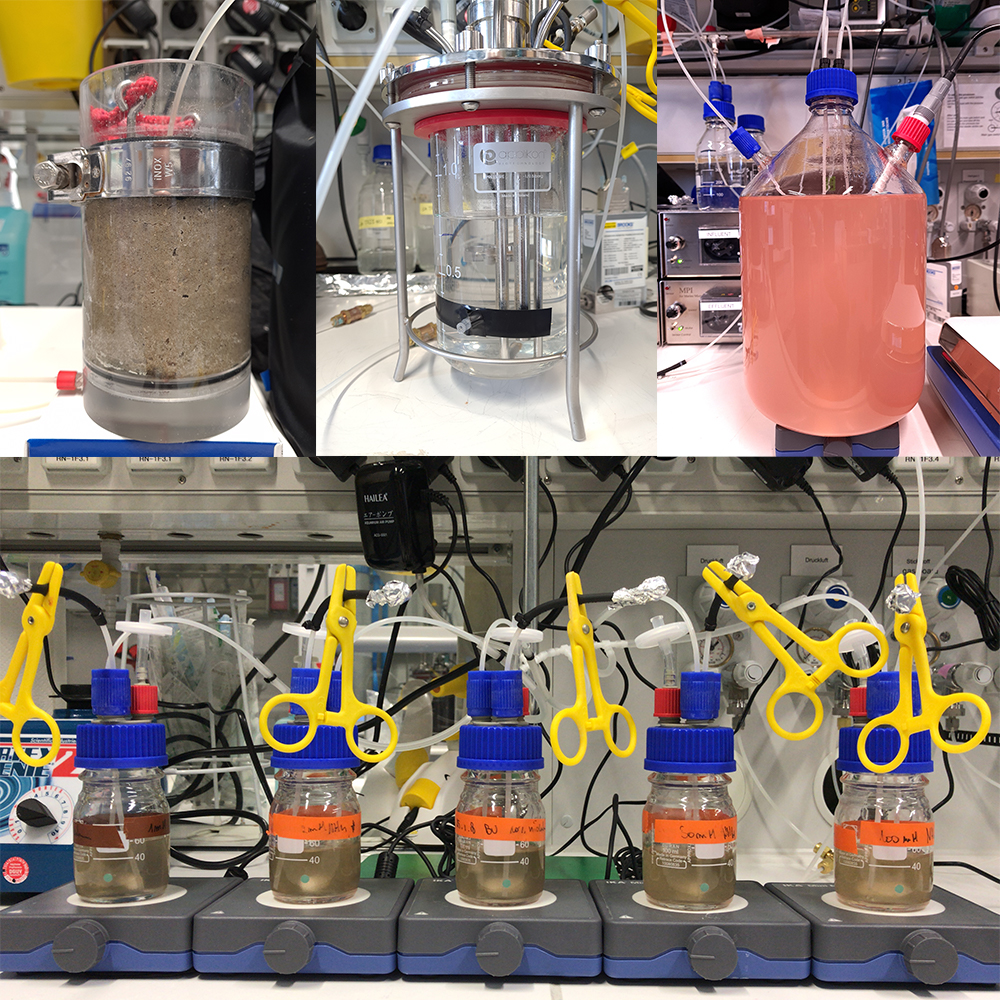
\includegraphics[scale=0.2]{Chemostat.jpg}
            \end{center}

            \normalsize{Un quimiostato es una buena opción para el cultivo de microorganismos, ya que establecemos condiciones que permanecen constantes, contra los cultivos hechos en lotes. Esto facilita enormemente la reproducción de los experimentos. Algunas de las utilidades del quimiostato son que puede ser utilizado en cultivos puros para el estudio de la cinética del crecimiento microbiano, o para enfoques ómicos más detallados. También se puede utilizar para experimentos de competición [1].}\\
            
            \normalsize{En estos experimentos se liberan en el recipiente dos o tres microorganismos diferentes, con nichos comparables en condiciones variables; con tasas de crecimiento altas o bajas; con concentraciones de oxígeno altas o bajas; distintos valores de pH o temperatura; con o sin factores de crecimiento, etc [1].}

            \subsubsection{GREENT}{

                \normalsize{La  actividad humana ha tenido serios impactos en los ciclos biológicos del carbono y nitrógeno, y como consecuencia, el calentamiento global y la contaminación del agua. En este contexto, las tecnologías relacionadas con el tratamiento de agua ha mejorado en las últimas décadas. En particular, el uso de anammox (bacterias anaeróbicas oxidantes de amonio) en gránulos con oxígeno tiene el potencial de convertir las tratadoras de agua en sistemas energéticamnete eficientes con mínima emisión de gases de efecto invernadero [1].}\\

                \normalsize{Existen microorganismos que acoplan la oxidación anaeróbica del metano con la desnitrificación. Una integración innovadora de estos en determinados sistemas de tratamiento de aguas podría ofrecer una solución elegante y eficiente para combatir las emisiones de gases de efecto invernadero de las mismas [1].}\\
                
                \normalsize{El propósito del \textit{GREENT}, o \textit{Mitigación de Gases de Efecto Invernadero Mediante Tecnología Avanzada de Eliminación de Nitrógeno} (por sus siglas en inglés) es determinar las emisiones de óxido nitroso en los bioreactores de nitritación parcial-anammox, y los parámetros que las gobiernan, e investigar las vías responsables con un detalle molecular. Aunado a ésto, también explorar la viabilidad de un bioreactor que elimine el amonio y metano de manera simultanea mediante anammox, y microorganismos anaeróbicos oxidantes de metano [1].}
            
            }
        
        }

        \subsection{Ecuación de Hamilton-Jacobi, Viscosidad y Constricciones.}
    
    }

    \vspace{0.2cm}
        \rule{150mm}{0.5mm} %%%%----- -----%%%%
    \vspace{0.2cm}

    \section{Modelo}{

        \subsection{Descripción del Entorno Biológico.}
        
        
        \normalsize{Consideremos un organismo que tiene que proporcionan energía (tales recursos se denominan sustituibles). Sean $S_1$ y $S_2$ las concentraciones de estos dos recursos contenidos en un quimiostato. Entonces el vector:}\\
        
        \begin{equation}
        I=\binom{S_{1}}{S_{2}},
        \end{equation}

        \normalsize{constituye la condición ambiental [7,8].}\\

        \normalsize{Los organismos pueden caracterizarse por diversos grados de consumir. Describimos estos rasgos por x y varían continuamente entre 0 y 1. Si el rasgo toma el valor 0, sólo se consume el recurso $S_2$ y cuando el rasgo toma el valor de 1 solo se consume el recurso $S_1$. El efecto general en el cual contribuyen los dos rasgos se describe a partir de los coeficientes $\eta(x)$  y $\xi(x)$, en el cual la cantidad promedio que consume un organismo con el rasgo x para los recursos 1 y 2 viene dado como:  $\eta(x)$ $S_1$ y $\xi(x)$ $S_2$ respectivamente.}\\

        \normalsize{En el caso de una población consumidora monomórfica, la dinámica ecológica está gobernada por el siguiente sistema de ecuaciones diferenciales:}\\

        \begin{equation}
        \begin{split}
             \frac{d S_1}{dx}&=S_{01}-S_1-\eta(x)S_1X\\  \frac{d S_2}{dx}&=S_{02}-S_2-\xi(x)S_2X\\ \frac{d S_1}{dx}&=-X+\eta(x)S_1X-\xi(x)S_2X 
        \end{split}
        \end{equation}

        \normalsize{Donde X representa la densidad de la población consumidora y $S_{01}$ es la concentración del recurso i en el medio de entrada.
        El sistema ecuaciones (2) tiene siempre que cumplir:}\\

        \begin{equation}
            \eta(x)S_1X-\xi(x)S_2X>1,
        \end{equation}

        \normalsize{y la tasa de crecimiento poblacional de los consumidores con el rasgo X, bajo condiciones ambientales constantes I, está dada por:}\\

        \begin{equation}
            r(x,I)=-1+\eta(x)S_1X+\xi(x)S_2X.
        \end{equation}

        \normalsize{Ahora, el análogo de (2) para la competencia de dos poblaciones consumidoras, una con el rasgo x y la otra con el rasgo y, está dado por el siguiente sistema:}\\

        \begin{equation}
        \begin{split}
            \frac{d S_1}{dt}&=S_{01}-S_1-\eta(x)S_1X_1-\eta(y)S_1X_2\\  \frac{d S_2}{dt}&=S_{02}-S_2-\xi(x)S_2X_1-\xi(y)S_2X_2\\ \frac{d X_1}{dx}&=-X_1+\eta(x)S_1X_1+\xi(x)S_2X_1\\
            \frac{d X_2}{dx}&=-X_2+\eta(y)S_1X_2+\xi(y)S_2X_1
        \end{split}
        \end{equation}

        \normalsize{En el estado estacionario, tanto como r(x,I) y r(y,I) son iguales a cero. Estas son dos ecuaciones lineales con dos incógnitas, $S_1$ y $S_2$. La solución se expresa como:}\\

        \begin{equation}
            \binom{S_1}{S_2}=\frac{1}{\eta(x)\xi(y)-\eta(y)\xi(x)}\binom{\xi(y)-\xi(x)}{\eta(y)-\eta(x)}
        \end{equation}

        
        \normalsize{A continuación, las dos relaciones de retroalimentación pueden utilizarse para deducir que las densidades en estado estacionario de las dos poblaciones consumidoras son:}\\

        \begin{equation}
            \binom{X_1}{X_2}=\frac{1}{\eta(x)\xi(y)-\eta(y)\xi(x)}\binom{\frac{\xi(y)S_{01}}{\xi(y)-\xi(x)}-\frac{\eta(y)S_{02}}{\eta(x)-\eta(y)}-\frac{\eta(y)-\xi(y)}{\eta(x)\xi(y)-\eta(y)\xi(x)}}{\frac{-\xi(x)S_{01}}{\xi(y)-\xi(x)}-\frac{\eta(x)S_{02}}{\eta(x)-\eta(y)}-\frac{\xi(x)-\eta(x)}{\eta(x)\xi(y)-\eta(y)\xi(x)}}
        \end{equation}

        \normalsize{De acuerdo con el Principio de Exclusión Competitiva, tres o más poblaciones consumidoras no pueden coexistir en estado estacionario utilizando solo dos recursos. De hecho, si r(x,I), r(y,I) y r(z,I) se igualan a cero, obtendremos tres ecuaciones lineales con solo dos incógnitas, lo que implica que, en general, no existe solución.}\\


        
        \subsection{Sistemas de Ecuaciones de Selección-Mutación y Paso al Límite para Mutaciones.}

        \normalsize{Si la reproducción no es completamente fiel, un consumidor con el rasgo yyy puede generar descendencia con el rasgo x. Sea K(x,y) la densidad de probabilidad correspondiente. En ese caso, se espera encontrar, con el tiempo, consumidores con todos los rasgos posibles. Sea n(t,.) la densidad de consumidores en el tiempo t. El sistema queda descrito por:}

        \begin{equation}
            \begin{split}
                \frac{d S_1(t,x)}{dt}&=S_{01}-S_1(t)+S_1(t)\int_{0}^{1}\eta(y)n(t,x)dx\\
               \frac{d S_1(t,x)}{dt}&=S_{02}-S_2(t)+S_2(t)\int_{0}^{1}\xi(x)n(t,x)dx\\
              \frac{d n(t,x)}{dt}&=-n(t,x)+\int_{0}^{1}K(x,y)[S_1(t)\eta(y)+S_2(t)\xi(x)]n(t,y)dy,
            \end{split}
        \end{equation}

        \normalsize{describe la interacción, a través de los recursos, de los diversos tipos de consumidores, así como el efecto de la mutación. Por lo tanto, se le denomina ecuación de selección-mutación (o sistema de ecuaciones). Por simplicidad, en la situación en la que la descendencia de un individuo con el rasgo x tiene una distribución de rasgos descrita por la densidad K(x,.).}\\

        \normalsize{Ahora, sea K(x,y) dependiente de un pequeño parámetro $\epsilon$; la idea es que las mutaciones son necesariamente pequeñas, lo cual incorporamos asumiendo que $K_\epsilon$ es insignificantemente pequeño para x fuera de un vecindario de radio $\epsilon$ alrededor de y [9].}\\

        \normalsize{Reescalamos el tiempo sustituyendo $\tau=\epsilon$t (este escalamiento ajusta la escala temporal de modo que, al hacer $\epsilon$ desaparecer, la escala de tiempo se adapte para observar el efecto de las mutaciones). Al escribir nuevamente t como $\tau$, ahora podemos reescribir la última ecuación de (4) como:}\\

        \begin{equation}
            \frac{\epsilon}{n(t,x)}\frac{d n(t,x)}{dt}=-1+\int_{0}^{1}K(x,y)[S_1(t)\eta(y)+S_2(t)\xi(x)]\frac{n(y,t)}{n(t,x)}dy.
        \end{equation}

        \normalsize{podemos luego realizar la siguiente transformación}\\

        \begin{equation}
            \varphi(t,x)=\epsilon ln[n(t,x)],
        \end{equation}

        \normalsize{mientras que el segundo término en el lado derecho puede escribirse como:}\\

        \begin{equation}
            \int_{0}^{1}K_{\epsilon}(x,y)[S_1(t)\eta(y)+S_2(t)\xi(x)]e^{\frac{\varphi(t,y)-\varphi(t,x)}{\epsilon}}dy
        \end{equation}

        \normalsize{Ahora supongamos que $K_{\epsilon}$ (x,y) es lo suficientemente pequeño para la variable y fuera de un vecindario de radio $\epsilon$ alrededor de x. Luego, realizamos el cambio de variable de integración y=x+$\epsilon$z y aproximamos:}\\

        \begin{equation}
            \frac{\varphi(t,y)-\varphi(t,x)}{\epsilon} \to \frac{d\varphi(t,x) }{dx}z
        \end{equation}

        \normalsize{Además, asumimos que la probabilidad de aparición de un nuevo rasgo como resultado de una mutación depende únicamente de la distancia al rasgo original. Por lo tanto, reemplazamos el kernel $K_{\epsilon}$ por un kernel de convolución $\widetilde{K}$ y aproximamos:}\\

        \begin{equation}
            K_{\epsilon}(x,y)dy\longrightarrow \widetilde{K}(z)dz

        \end{equation}

        \normalsize{Donde K es una función no negativa y par definida en (− \infty, \infty),cuya integral es igual a 1.Al tomar formalmente el límite cuando $\epsilon$ tiende a 0 en (9), obtenemos:}\\


        
        \subsection{Descripción Superficial del Modelo Numérico.}
          \subsection{Descripción del Método numérico}
\subsubsection{Diferencias finitas}

    Es un método numérico para la solución de ecuaciones diferenciales, se basa en la discretización de las variables dependientes e independientes convirtiendo las ecuaciones continuas en sistemas algebraicos más fáciles de resolver.

    Es una técnica útil para la solución de sistemas complejos. Consiste en aproximar las derivadas de las ecuaciones mediante \textbf{diferencias finitas}, esto es, que se reemplaza la derivada de una función en términos continuos por una expresión algebraica que involucra a la función en puntos discretos en una malla de tiempo, espacio, etc.

    \textbf{{Cómo funciona el Método de Diferencias Finitas}}
        \begin{enumerate}
            \item Discretización.

                Se discretizan las variables independientes en una malla, y las soluciones se calculan en algún punto de la malla

            \item Aproximación de Derivadas

                Las derivadas de las funciones se reemplazan por diferencias finitas en cada punto de la malla. Este reemplazo se hace dependiendo del problema

            \item Ecuaciones algebraicas

                Al reemplazar las derivadas por diferencias finitas, se obtienen ecuaciones algebraicas fáciles de resolver

            \item Iteración

                El sistema de ecuaciones se resuelve de manera iterativa, los valores de la solución en cada punto de la malla se calculan por pasos hasta obtener una solución en todo el dominio
        \end{enumerate}
        
        Este método presenta algunas ventajas y desventajas: simplicidad ya que es fácil de implementar, aplicación, es aplicable a problemas de difusión, reacción, etc. Por otro lado, tiene como inconveniente que: el error es inversamente proporcional al tamaño de la malla, pero si se hace la malla más pequeña, tiene más costo computacional, si los pasos temporales son grandes, esto puede ocasionar que la solución no sea estable\footnote{Que el método sea inestable se refiere a que el error en la solución crece conforme el tiempo}.

    \subsubsection{Diferencias finitas Semi-Implicito}

        Se usa para la solución de sistemas de ecuaciones diferenciales en los que aparecen fenómenos de difusión y reacción. Es un método que involucra la solución combinando dos métodos explicito e implícito, y el método es estable.

        \textbf{Explicito:} las variables en el paso de tiempo se calculan en el paso actual con la información del paso anterior, este es inestable en algunas ecuaciones.

        \textbf{Implicito:} las variables en el paso de tiempo se calculan en el siguiente paso, este es más costoso computacionalmente, pero es más estable

    \subsection{Aplicación a la ecuación de Selección-Mutación}
    \subsubsection{Simulación directa}

    La ecuación de Selección-Mutación \eqref{??} de forma discreta es
    \begin{equation}
        \left\{\begin{matrix}
            S_{i}^{(k+1)} = &  S_{i}^{0}-\Delta tS_{i}^{(k+1)}[1+\langle{n^{(k)}\eta_{i}}\rangle  ] \\
            n_{j}^{(k+1)} = &  n_{j}^{(k)}-\Delta t n_{j}^{(k+1)}+\Delta t([S_{1}^{(k+1)}\eta+S_{2}^{(k+1)}\xi]n^{(k)}\star \tilde{K})_{j}
        \end{matrix}\right.
    \label{eq:S-M_dis}
    \end{equation}

    donde 
    \begin{equation*}
        \langle{n^{(k)}\eta_{i}}\rangle = \frac{1}{N}\sum_{j=1}^{N}n_{j}^{(k)}\eta_{j}
    \end{equation*}

    \begin{equation*}
        (\eta n^{(k)}\star \tilde{K})_{j}=\frac{1}{2M+1}\sum_{m=-M}^{M}\eta_{j-m}n_{j-m}^{(k)}\tilde{K}_{M}
    \end{equation*}

    el primer término de la \eqref{eq:S-M_dis} representa la dinámica de los nutrientes, el segundo término se refiere a la dinámica de los consumidores, $\langle{n^{(k)}\eta_{i}}\rangle$ es el promedio de la densidad de consumidores por su capacidad de consumir uno de los nutrientes, y $(\eta n^{(k)}\star \tilde{K})_{j}$ es la operación de convolución, este modula las interacciones de los consumidores en el espacio discreto del rasgo $x$, $y$

    \subsubsection{Aproximación Hamilton-Jacobi}

    



%%_________________________________________________________________________________________________________________________________________________________%%
    }

    \vspace{0.2cm}
        \rule{150mm}{0.5mm} %%%%----- -----%%%%
    \vspace{0.2cm}

    \section{Ejemplos}{

        \subsection{Tumores}

        \subsection{Osos-Salmones}
    
    }

    \vspace{0.2cm}
        \rule{150mm}{0.5mm} %%%%----- -----%%%%
    \vspace{0.2cm}

    \section{Conclusiones y Comentarios Finales}

    \vspace{0.2cm}
        \rule{150mm}{0.5mm} %%%%----- -----%%%%
    \vspace{0.2cm}

    \section{Apéndices}

    \vspace{0.2cm}
        \rule{150mm}{0.5mm} %%%%----- -----%%%%
    \vspace{0.2cm}

    %%%%%%%%%%%%%%%%%%%%%%%%%% call al archivo de bibliografia
    	\bibliography{referencias.bib}
%%%%%%%%%%%%%%%%%%%%%%%%
    \section{Bibliografías}

    \begin{enumerate}
        \item {

            \normalsize{Chemostat. (s.f.). Max Planck Institute For Marine Microbiology. Recuperado 21 de noviembre de 2024, de https://www.mpi-bremen.de/en/Chemostat.html}

        }

        \item {

            \normalsize{Monge-Nájera, J. (2002). Biología general. EUNED. ISBN 9789968311892. Consultado el 25 de noviembre de 2024.}
        
        }

        \item{
            \normalsize{Calvez, V., Lam, K.-Y. (2020) . Uniqueness of the viscosity solution of a constrained Hamilton–Jacobi equation. SPRINGER, 1-2. https://doi.org/10.1007/s00526-020-01819-0} 
        }

        \item {
            \normalsize{Barles, G., Perthame, B. (2007). Concentrations and constrained Hamilton-Jacobi equations arising in adaptive dynamics. Contemporary Mathematics, 439, 57-68.}
        }

        \item{
            \normalsize{Mirrahimi, S., Perthame, B., Bouin, E., Millien, P. (2011). Population formulation of adaptative meso-evolution: theory and numerics. The mathematics of Darwin’s legacy, 159-174.}
        }

        \item{
            \normalsize{De la Calleja, E. M., Carrillo, J. L., Santamaría-Holek, I. (2016). Bragg-Williams approximation for the dynamics of prey-predator biological associations. arXiv preprint arXiv:1603.03608.}
        }
    \end{enumerate}

\end{document}
